\chapter{The Fundamental Group}
\section{The Fundamental Grupoid}

\begin{lemma}[Gluing Lemma]
	Let $X,Y \in \ob(\mathsf{Top})$, $(X_\alpha)_{\alpha \in A}$ a finite closed cover of $X$ and $(f_\alpha)_{\alpha \in A}$ a finite family of maps $f_\alpha \in \mathsf{Top}(X_\alpha,Y)$ such that $f_\alpha\vert_{X_\alpha \cap X_\beta} = f_\beta\vert_{X_\alpha \cap X_\beta}$ for all $\alpha,\beta \in A$. Then there exists a unique $f \in \mathsf{Top}(X,Y)$ such that $f\vert_{X_\alpha} = f_\alpha$ for all $\alpha \in A$.
	\label{lem:gluing_lemma}
\end{lemma}

\begin{proof}
	Let $x \in X$. Since $(X_\alpha)_{\alpha \in A}$ is a cover of $X$, we find $\alpha \in A$ such that $x \in X_\alpha$. Define $f(x) := f_\alpha(x)$. This is well defined, since if $x \in X_\alpha \cap X_\beta$ for some $\beta \in A$, we have that $f(x) = f_\beta(x) = f_\alpha(x)$. Clearly $f\vert_{X_\alpha} = f_\alpha$ for all $\alpha \in A$ and $f$ is unique. Let us show continuity. To this end, let $K \subseteq Y$ be closed. Then 
	\begin{align*}
		f^{-1}(K) &= X \cap f^{-1}(K)\\
		&= \bigcup_{\alpha \in A} X_\alpha \cap f^{-1}(K)\\
		&= \bigcup_{\alpha \in A} \del[1]{X_\alpha \cap f^{-1}(K)}\\
		&= \bigcup_{\alpha \in A} \del[1]{X_\alpha \cap f_\alpha^{-1}(K)}. 
	\end{align*}
	Since each $f_\alpha$ is continuous, $f_\alpha^{-1}(K)$ is closed in $X_\alpha$ for each $\alpha \in A$ and thus since $X_\alpha$ is closed, $f^{-1}(K)$ is closed as a finite union of closed sets.
\end{proof}

\begin{theorem}
	There is a functor $\mathsf{Top} \to \mathsf{Grpd}$. 
\end{theorem}

\begin{proof}
	The proof is divided into several steps. Let us denote $\Pi : \mathsf{Top} \to \mathsf{Grpd}$ for the claimed functor.
	\begin{enumerate}[label = \textit{Step \arabic*:},wide = 0pt, itemsep = 1.5ex]
		\item \textit{Definition of $\Pi$ on objects.} Let $X,Y \in \ob(\mathsf{Top})$, $f,g \in \mathsf{Top}(X,Y)$ and $A \subseteq X$. A map $F \in \mathsf{Top}(X \times I,Y)$ is called a \bld{homotopy from $X$ to $Y$ relative to $A$}, if 
			\begin{itemize}[leftmargin = *]
				\item $F(x,0) = f(x)$, for all $x \in X$.
				\item $F(x,1) = g(x)$, for all $x \in X$.
				\item $F(x,t) = f(x) = g(x)$, for all $x \in A$ and for all $t \in I$.
			\end{itemize}
			If there exists a homotopy between $f$ and $g$ relative to $A$ we say that $f$ and $g$ are \bld{homotopic relative to $A$} and write $f \simeq_A g$. If we want to emphasize the homotpoy relative to $A$, we write $F : f \simeq_A g$.

			\begin{lemma}
				Let $X,Y \in \ob(\mathsf{Top})$ and $A \subseteq X$. Then being homotopic relative to $A$ is an equivalence relation on $\mathsf{Top}(X,Y)$.
			\end{lemma}

			\begin{proof}
				Define a binary relation $R_A \subseteq \mathsf{Top}(X,Y) \times \mathsf{Top}(X,Y)$ by
				\begin{equation*}
					f R_A g \quad :\Leftrightarrow  \quad f \simeq_A g.
				\end{equation*}
				Let $f \in \mathsf{Top}(X,Y)$. Define $F \in \mathsf{Top}(X\times I,Y)$ by 
				\begin{equation*}
				F(x,t) := f(x).
				\end{equation*}
				Then clearly $F : f \simeq_A f$. Hence $R_A$ is reflexive.\\
				Let $g \in \mathsf{Top}(X,Y)$ and assume that $f R_A g$. Thus $G : f \simeq_A g$. Define $F \in \mathsf{Top}(X \times I,Y)$ by
				\begin{equation*}
					F(x,t) := G(x,1-t).
				\end{equation*}
				Then it is easy to check that $F : g \simeq_A f$ and so $R_A$ is symmetric.\\
				Finally, let $h \in \mathsf{Top}(X,Y)$ and suppose that $f R_A g$ and $g R_A h$. Hence $F_1 : f \simeq_A g$ and $F_2 : g \simeq_A h$. Define $F \in \mathsf{Top}(X\times I,Y)$ by
				\begin{equation*}
					F(x,t) := \ccases{
						F_1(x,2t) & 0 \leq t \leq \frac{1}{2},\\
						F_2(x,2t-1) & \frac{1}{2} \leq t \leq 1.
					}
				\end{equation*}
				Continuity of $F$ follows by an application of the gluing lemma \ref{lem:gluing_lemma}. Then it is easy to check that $F : f \simeq_A h$ and hence $R_A$ is transitive.
			\end{proof}

			Let $X \in \ob(\mathsf{Top})$ and $u$ a path in $X$ from $p$ to $q$. Define the \bld{path class $\sbr{u}$ of $u$} by $\sbr{u} := \sbr{u}_{R_{\partial I}}$. Define now
			\begin{itemize}[leftmargin = *]
				\item $\ob\del[1]{\Pi(X)} := X$.
				\item $\Pi(X)(p,q) := \cbr{\sbr{u} : \text{$u$ is a path from $p$ to $q$}}$ for all $p,q \in X$.
				\item Let $p \in X$. Then define $\id_p \in \Pi(X)(p,p)$ by $\id_p := \sbr[0]{c_p}$, where $c_p$ is the constant path defined by $c_p(s) := p$ for all $s \in I$.
				\item And $\Pi(X)(q,r) \times \Pi(X)(p,q) \to \Pi(X)(p,r)$ by 
					\begin{equation*}
						(\sbr{v}, \sbr{u}) \mapsto \sbr{u \ast v}
					\end{equation*}
					Where $u \ast v \in \mathsf{Top}(p,r)$ is the \bld{concatenated path of $u$ and $v$}, defined by
					\begin{equation*}
						(u \ast v)(s) := \ccases{
							u(2s) &    0 \leq t \leq \frac{1}{2},\\
							v(2s - 1) & \frac{1}{2} \leq t \leq 1
						}.
					\end{equation*}
					Continuity follows again from the gluing lemma \ref{lem:gluing_lemma} whereas well definedness follows from the next lemma.

					\begin{lemma}
						Suppose that $\sbr{u_1},\sbr{u_2} \in \Pi(X)(p,q)$ and $\sbr{v_1},\sbr{v_2} \in \Pi(X)(q,r)$ such that $\sbr{u_1} = \sbr{u_2}$ and $\sbr{v_1} = \sbr{v_2}$. Then $\sbr{u_1 \ast v_1} = \sbr{u_2 \ast v_2}$.
					\end{lemma}

					\begin{proof}
						By assumption we have $G : u_1 \simeq_{\partial I} u_2$ and $H : v_1 \simeq_{\partial I} v_2$. Define $F \in \mathsf{Top}(I \times I,X)$ by
						\begin{equation*}
							F(s,t) := \ccases{
								G(2s,t) & 0 \leq s \leq \frac{1}{2},\\
								H(2s - 1,t) & \frac{1}{2} \leq s \leq 1.
							}
						\end{equation*}
						Again, continuity follows from the gluing lemma \ref{lem:gluing_lemma} and it is easy to check that $F : u_1 \ast v_1 \simeq_{\partial I} u_2 \ast v_2$.
					\end{proof}
			\end{itemize}

			Let us now check that $\Pi(X)$ is indeed a category. 
			
			
			Let $\sbr{u} \in \Pi(X)(p,q)$. We want to show that $u \simeq_{\partial I} c_p \ast u$. To this end, we consider figure \ref{fig:unit_axiom} and conclude that a suitable homotopy is given by $F \in \mathsf{Top}(I \times I,X)$ defined by
			\begin{equation*}
				F(s,t) := \ccases{
					p & 0 \leq 2s \leq t,\\
					\displaystyle u\del[3]{\frac{2s - t}{2 - t}} & t \leq 2s \leq 2.
				}
			\end{equation*}
			\begin{figure}[h!tb]
				\centering
				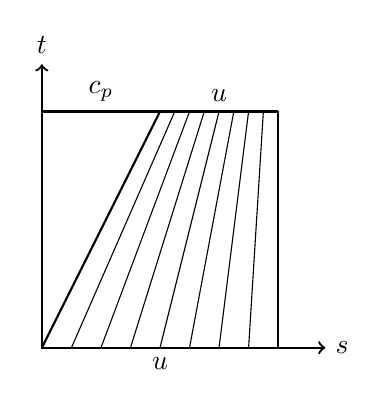
\begin{tikzpicture}[scale = 3]
    				% Draw axes
    				\draw [<->,thick] (0,1.2) node[above] {$t$}
        			|- (1.2,0) node[right] {$s$};
    				% Draw two intersecting lines
					\draw [thick] (0,0) -- (.5,1);
					\draw [thick] (0,1) -- (1,1);
					\draw [thick] (1,0) -- (1,1);

					\draw [thin] (.25,0) -- (.625,1);
					\draw [thin] (.125,0) -- (.5625,1);
					
					\draw [thin] (.5,0) -- (.75,1);
					\draw [thin] (.375,0) -- (.6875,1);
					\draw [thin] (.625,0) -- (.8125,1);
					\draw [thin] (.875,0) -- (.9375,1);
					\draw [thin] (.75,0) -- (.875,1);
					
					
					\draw (.5,0) node[below] {$u$};
					\draw (.25,1) node[above] {$c_p$};
					\draw (.75,1) node[above] {$u$};
			\end{tikzpicture}
			\caption{$u \simeq_{\partial I} c_p \ast u$.}
			\label{fig:unit_axiom}
			\end{figure}
			Similarly, considering figure \ref{fig:associativity_axiom} leads to $F \in \mathsf{Top}(I \times I,X)$ defined by
			\begin{equation*}
				F(s,t) := \ccases{
					\displaystyle u\del[3]{\frac{4s}{t + 1}} & -1 \leq 4s - 1 \leq t,\\
					\displaystyle v(4s - t - 1) & t \leq 4s - 1 \leq t + 1,\\
					\displaystyle w\del[3]{\frac{4s - t - 2}{4 - t - 2}} & t + 1 \leq 4s - 1 \leq 3.
				}
			\end{equation*}
			\begin{figure}[h!tb]
				\centering
				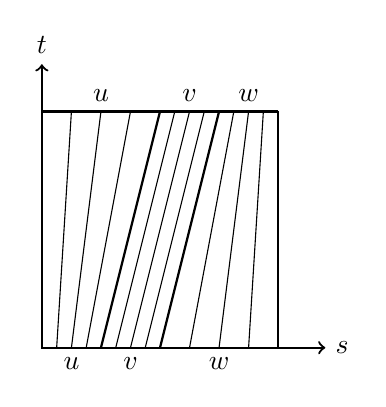
\begin{tikzpicture}[scale = 3]
    				% Draw axes
    				\draw [<->,thick] (0,1.2) node[above] {$t$}
        			|- (1.2,0) node[right] {$s$};
    				% Draw two intersecting lines
					\draw [thick] (.25,0) -- (.5,1);
					\draw [thick] (.5,0) -- (.75,1);
					\draw [thick] (0,1) -- (1,1);
					\draw [thick] (1,0) -- (1,1);
					
					\draw [thin] (.125,0) -- (.25,1);
					\draw [thin] (.0625,0) -- (.125,1);
					\draw [thin] (.1875,0) -- (.375,1);
					
					\draw [thin] (.375,0) -- (.625,1);
					\draw [thin] (.3125,0) -- (.5625,1);
					\draw [thin] (.4375,0) -- (.6875,1);

					\draw [thin] (.75,0) -- (.875,1);
					\draw [thin] (.625,0) -- (.8125,1);
					\draw [thin] (.875,0) -- (.9375,1);

					\draw (.125,0) node[below] {$u$};
					\draw (.375,0) node[below] {$v$};
					\draw (.75,0) node[below] {$w$};
					
					\draw (.25,1) node[above] {$u$};
					\draw (.625,1) node[above] {$v$};
					\draw (.875,1) node[above] {$w$};
			\end{tikzpicture}
			\caption{$(u \ast v) \ast w \simeq_{\partial I} u \ast (v \ast w)$.}
			\label{fig:associativity_axiom}
			\end{figure}
			
			Lastly, we check that $\Pi(X)$ is a grupoid. To this end, for a path $u$ from $p$ to $q$, define its \bld{reverse path $\wbar{u}$} by
			\begin{equation*}
				\wbar{u}(s) := u(1 - s). 
			\end{equation*}
			We claim that $u \ast \wbar{u} \simeq_{\partial I} c_p$.
	\end{enumerate}
\end{proof}

\section{The Fundamental Group}

\begin{lemma}
	Let $\mathcal{\altG}$ be a locally small grupoid. Then for every $X \in \ob(\mathcal{\altG})$, $\mathcal{\altG}(X,X)$ can be equipped with a group structure.	
\end{lemma}

\begin{proof}
	Since $\mathcal{\altG}$ is locally small, $\mathcal{\altG}(X,X)$ is a set for every $X \in \ob(\mathcal{\altG})$. Define a multiplication $\mathcal{\altG} \times \mathcal{\altG} \to \mathcal{\altG}$ by $gh := h \circ g$. 
\end{proof}
